\documentclass{article}
\usepackage{amsmath, amssymb, amsthm}
\usepackage{hyperref}
\usepackage{fullpage,fancyhdr}
\usepackage{graphicx}
\usepackage{algorithmic}

\pagestyle{fancy}
​
\renewcommand\headheight{20pt}
​
\chead{\Large ISL Notes}
​
\renewcommand{\headrulewidth}{0.4pt}
\renewcommand{\footrulewidth}{0.4pt}
\newcommand{\R}[0]{\mathbb{R}}
\DeclareMathOperator{\tr}{tr}
\DeclareMathOperator{\Cut}{Cut}
\renewcommand{\labelenumi}{\alph{enumi})}
\parindent 0in
\parskip .1in
Author: Devin Kreuzer\\
Based on \textit{An Introduction to Statistical Learning} by James, Witten, Hastie and Tibshirani.
\begin{document}\\
\\
\section{Metrics}

Recall:\[\frac{TP}{TP+FN}\]
Interpretation: We want very few False Negatives. We don't want to miss any positives. Lower confidence on positives, but more likely to catch all of them.\\
\\
Precision:\[\frac{TP}{TP+FP}\]
Interpretation: We want very few False Positives. We want to be sure about our positives. High confidence on our positives, but may not have caught all of them.


\section{Statistical Learning}

\subsection{Parametric Models}
\begin{description}

  \item[$\bullet$] Advantage is fewer parameters to learn and model interpretability.

  \item[$\bullet$] Disadvantage is the assumption itself: fixed model.

\end{description}

\subsection{Non-parametric Models}
\begin{description}

  \item[$\bullet$] Advantage is potential to accurately fit wider range of shapes for $f$.

  \item[$\bullet$] Disadvantage is model needs for more training instances to be able to estimate $f$ and loss of model interpretability.

\end{description}

\subsection{Bias, Variance, Model Complexity (from ELS)}
\begin{description}

  \item[$\bullet$] We assume that $Y=f(x) + \epsilon$ where $f$ represents the best possible learned model. There is noise in the learned model $\hat{f}$ coming from the set $T$ it is trained on. We are interested in models $\hat{f}$ that are close to $f$ and models $\hat{f}$ that do not vary drastically in response to the specific training set $T$ it is trained on. This is the gist of bias-variance trade-off. Mathematically:
  
  \[Err(x) = \mathbb{E}[(Y-\hat{f}(x))^2|X=x] = \mathbb{E}[(f(x) + \epsilon -\hat{f}(x))^2|X=x]\]
  \[ = (\mathbb{E}[\hat{f}(x)] - f(x))^2 + \mathbb{E}[\hat{f}(x) - \mathbb{E}[\hat{f}(x)]]^2 + \sigma^2\]
  
  The first term can be thought of as how much is the expected model (stochasticity comes from training on different training sets) differing from the best possible model. The second term can be thought of as how sensitive/robust is my model to fluctuations in sets it is trained on.
  

\end{description}

\section{Model Assessment and Selection}

\subsection{Cross-Validation}

\begin{description}

  \item[$\bullet$] Given models $f(x,\alpha)$ where $x$ denotes training set and $\alpha$ are hyperparameters, let $f^{-k}(x,\alpha)$ denote the $\alpha$th model trained without the $k$th part. We select the final chosen model $f(x,\hat{\alpha})$ fit on the whole training set based on the minimum $\hat{\alpha}$ which minimizes:
  
  \[CV(f, \alpha) = \frac{1}{N}\sum_{i=1}^N L(y_1, f^{-k(i)}(x_i))\]
  
  This more effectively estimates the average error Err = $\mathbb{E}[L(Y,f(X))]$
  
  \item[$\bullet$] Selecting $K=N$ most effectively estimates the $\mathbb{E}[L(Y,f(X))]$, but the best estimator can have very high variance due to training on such similar sets (will tend to overfit training data, still). Also has higher computational burden.
  
  \item[$\bullet$] Selecting low $K$ will produce an estimator with a lower variance, but potentially higher bias model, since the model was trained on much fewer data points.
  
  \item[$\bullet$] K typically depends on the learning curve. If the learning curve has a high slope at the given training size for $K$, cross-validation will overestimate prediction error (higher MSE, lower AUC).
  
  \item[$\bullet$] Model selection without nested CV uses the same data to tune model parameters and evaluate model performance. Information may thus “leak” into the model and overfit the data. 
  \item[$\bullet$] Use nested cross validation to get better estimate of true prediction accuracy, but use cross-validation to actually find the final model. 

\end{description}

\section{Loss functions}

\subsection{Cross-Entropy Loss/Negative log-likelihood/Maximum Likelihood}
\begin{description}

  \item[$\bullet$] Straight-forward:
  
  \[\sum_i -(y_i\log(p_i) + (1-y_i)\log(1-p_i))\]
  
  The intuition is to bring the probabilities of belonging to a class as close to 1 as possible. As $p_i$ approach 1, the loss function converges to zero. Using log has a large advantage to counteract the saturation of large absolute values output by activation functions (vanishing gradient problem).
  

\end{description}


\section{Linear Regression}
\subsection{Multivariate Regression}

\begin{description}

  \item[$\bullet$] Can fit $\beta$ analytically or with gradient descent. 
  
  \item[$\bullet$] $\text{Var}(\hat{\beta}) = (\boldsymbol{X^TX})^{-1}\sigma^2$, where $\sigma^2$ is the variance of $y_i$ which can be estimated with $\hat{\sigma}^2 = \frac{1}{N-p-1}\sum_i(y_i - \hat{y_i})^2$
  
  \item[$\bullet$] To test hypothesis of specific coefficient $\beta_j$, compute Z-score:
  \[z_j = \frac{\hat{\beta}_j}{\hat{\sigma}\sqrt{v_j}}\]
  where $v_j$ is the $j$th diagonal element of $\bold{(X^TX})^{-1}$
  
  \item[$\bullet$] We assume $z$ is distributed as $t_{N-p-1}$ ($t$ distribution with $N-p-1$ degrees of freedom). However, if $\sigma$ is known instead of estimated, $z$ would have a standard normal distribution. Compute p-value to reject or accept null hypothesis $\beta_j=0$
  
  \item[$\bullet$] For computing significance of groups of coefficients simultaneously, compute $F$ statistic:
  \[F = \frac{(RSS_0 - RSS_1)/(p_1 - p_0)}{RSS_1/(N-p-1)}\]
  where $RSS_1$ is RSS for model with more features $(p_1+1)$ and $RSS_0$ is RSS for model with less features $(p_0+1)$. Under the null hypothesis that the smaller $RSS_0$ model is correct, $F$ follows an $F_{p_1-p_0, N-p-1}$ distribution.
  
  \item[$\bullet$] To obtain $95\%$ confidence intervals around $\beta_j$, we can report
  \[(\hat{\beta_j}-1.96\sqrt{v_j}\hat{\sigma}, \hat{\beta_j}+1.96\sqrt{v_j}\hat{\sigma})\]
  where we cn replace 1.96 for varying confidence intervals.
\end{description}

\subsection{Ridge Regression}

\begin{description}

  \item[$\bullet$] When using many correlated variables in a linear regression, coefficients are poorly determined and exhibit high variances.
  
  \item[$\bullet$] Ridge regression: need to standardize inputs before solving.
  
  \item[$\bullet$] The solution for $\beta_{ridge}$ is given by
  \[\hat{\beta}_{ridge} = \mathbf{(X^TX + \lambda I)^{-1}X^Ty}\]
  
  which actually renders the inversion nonsingular (invertible) if $X^TX$ is singular (noninvertible).
  
  \item[$\bullet$] Taking the SVD of $\bold{X = UDV^T}$, we can substitute this into the ridge regression solutions and observe the following:
  
  \[\bold{X}\beta = \bold{X(X^TX + \lambda I)^{-1}X^Ty}\]
  \[= \bold{UD(D^2 + \lambda I)^{-1}DU^Ty}\]
  \[= \bold{\sum_{j=1}^p u_j\frac{d_j^2}{d_j^2+\lambda}u_j^Ty}\]
  
  Ridge regression computes the coordinates of $y$ wrpt to orthonormal basis of $U$, and then shrinks these coordinates by a factor of $\frac{d_j^2}{d_j^2 + \lambda}$. $u_1$ is the normalized first principal components, and thus we apply the least amount of penalization in this direction.
  \[\text{Var}[\bold{X}v_1] = \text{Var}[\bold{u_1}d_1] = \frac{d_1^2}{N}\]
    
\end{description}

\subsection{Partial Least Squares}

\begin{description}

  \item[$\bullet$] Find linear combinations of feature space as so:
  \[\bold{z_1} = \sum_j \langle \bold{x_j}, \bold{y}\rangle\bold{x_j}\]
  
  inputs are weighted by their univariate strength of $\bold{y}$. We then regress $\bold{y}$ onto this direction to find the coefficient, and repeat procedure by orthogonalizing all $x$ with $z_1$ repeatedly.
\end{description}

\section{Tree-based methods}
\subsection{Regression}

\begin{description}

  \item[$\bullet$] Predict mean value of region belonging to.
  
    \item[$\bullet$] Make splits on recursive binary splitting: select \textbf{feature and threshold} which minimize RSS: squared difference between values and mean value in their region:
    
    \[\sum_j \sum_{i \in R_j} (y_i - \hat{y}_R{_j})^2\]
  
    \item[$\bullet$] Prune with Cost Complexity Pruning/Weakest Link Pruning: minimize RSS with added $|T|$ term (number of leaves/regions):
    
    \[\sum_j \sum_{i \in R_j} (y_i - \hat{y}_R{_j})^2 + \alpha|T|\]
    
    which generates new pruned trees for varying $\alpha$
\end{description}

\subsection{Classification}

\begin{description}

  \item[$\bullet$] Predict most occurring class in region.

  \item[$\bullet$] Two common criteria for splitting: Gini index (G) and Entropy (D). Let $p_{mk}$ denote proportion of observations from class $k$ in region $m$:
 
  \[G = \sum_k p_{mk}(1-p_{mk})\]
  \[D = -\sum_k p_{mk}\log p_{mk}\]
  
  which both approach 0 for $p_k$ approaching 0 or 1.

\end{description}

\subsection{Simple Trees vs. Linear Models}

\begin{description}

  \item[$\bullet$] Trees can only generate decision boundaries orthogonal to input space. The form of the decision boundary is important.
    \item[$\bullet$] Trees are generally very interpretable.
    \item[$\bullet$] Trees are mostly inferior for their lack of \textbf{robustness (high variance)}: small changes in input can lead to large changes in output.

\end{description}

\subsection{Bagging/Bootstrap Aggregation}

\begin{description}

    \item[$\bullet$] Bagging \textbf{uses} Bootstrapping! 
  
    \item[$\bullet$] Train on $B$ distinct bootstrapped training sets and average the predicted result from each model. 
    
     \item[$\bullet$] Used to \textbf{reduce variance/increase robustness} of trees (without pruning)
     
     \item[$\bullet$ Out of Bag Prediction] Each model has an expected $\frac{2}{3}$ of the training samples in it (from resampling). Predict $i$-th variable using the expected $\frac{B}{3}$ models that are not including it.
\end{description}

\subsection{Variable importance}

\begin{description}


      \item[$\bullet$] For single tree models, just see which features were first used in split.
      
      \item[$\bullet$] In bagging regression trees, record total amount that the RSS is decreased due to splits using the given predictor, averaged over $B$ trees. Large value indicates important predictor.
      
      \item[$\bullet$] In bagging classification trees, sum total amount of decrease in Gini index, averaged over $B$ trees.

\end{description}


\subsection{Random Forests}

\begin{description}

      \item[$\bullet$] Same as bagging, but also only consider a \textbf{random sample of predictors} for each split. Typical sample size is $\sqrt{p}$.
      
      \item[$\bullet$] Rationale: induce even more variance across the $B$ different trees. Random Forests reduce to Bagging if $m=p$ samples are chosen.
\end{description}

\subsection{Boosting}

\begin{description}

      \item[$\bullet$] In bagging, trees are built separately. In boosting, trees are grown \textbf{sequentially}. Goal is to slowly improve model to predict in regions it is not predicting well.
      
      \item[$\bullet$] Instead of fitting to outcomes $Y$, we fit small trees to the residuals output by previous fitted model and add this model to the function.
      
    \item[$\bullet$] Three tuning parameters: number of trees $B$, learning rate $\lambda$ and tree depths $d$.
    
    \item[$\bullet$] Output of model becomes
    \[\hat{y} = \lambda f_1(x) + \lambda f_2(x) + ... + \lambda f_B(x)\]
    
    

\end{description}

\newpage

\section{Support Vector Machines}

\subsection{Maximal Margin Classifier/Hard Margin Classifier}

\begin{description}
    \item[$\bullet$]For linear decision boundaries.
    \item[$\bullet$] Solve following constrained optimization problem:
    \[\max M\]
    \[\sum_j \beta_j^2 = 1\]
    \[y_i(\beta_0 + \beta_1x_{i1} + ... + \beta_px_{ip}) \geq M\]
    
    Intuition: force norm of \textbf{$\beta$} to be 1 to maintain notion of distance between hyperplane and $x$.
    
    \item[$\bullet$] Prone to overfitting (lacks robustness). Small changes in input near the boundary can completely modify model.
    
     \item[$\bullet$] Unique property of MMC: completely robust to some observations (non-support vectors).
    
\end{description}

\subsection{Support Vector Classifier/Soft Margin Classifier}

\begin{description}
    \item[$\bullet$] For linear decision boundaries.
    
    \item[$\bullet$] Allow some mistakes to increase robustness. Less overfitting:
    
        \[\max M\]
    \[\sum_j \beta_j^2 = 1\]
    \[y_i(\beta_0 + \beta_1x_{i1} + ... + \beta_px_{ip}) \geq M(1-\epsilon_i)\]
    \[\epsilon\geq 0, \sum_i \epsilon_i \leq C\]
    
    \item[$\bullet$] $\epsilon_i$ have important function: they tell us where the variable $i$ is located. If $\epsilon_i=0$, $i$ is on the right side of margin. If $\epsilon>0$, it is within the margin. If $\epsilon>1$, it is on the wrong side of the hyperplane.
    
    \item[$\bullet$] $C$ is a hyperparameter determining the budget of $\epsilon_i$. Controls bias/variance trade-off.
    
     \item[$\bullet$] Important concept: only observations with $\epsilon>0$ affect hyperplane (support vectors). High $C$ generates more support vectors (less sensitivity).
     
     \item[$\bullet$] Unique property of SVC: completely robust to some observations (non-support vectors).
     
       \item[$\bullet$] Classifying function becomes
       \[f(x) = \beta_0 + \sum_i \alpha_i \langle x,x_i \rangle\]
       Where $\alpha_i=0$ for non-support vectors.
\end{description}

\subsection{Support Vector Machines}

\begin{description}
    \item[$\bullet$] Extension of SVC using kernels to extend feature space. Linear in transformed space $\longrightarrow$ non-linear in original space.
    
    \item[$\bullet$] SVM combines SVC with non-linear kernel
    \[f(x) = \beta_0 + \sum_{i \in S} \alpha_i K(x,x_i)\]
    
    \item[$\bullet$] Example of polynomial kernel:
    \[K(x_i,x_j) = (1+\sum_k x_{ik}x_{jk})^d\]
    
    \item[$\bullet$] Example of radial kernel:
    \[K(x_i,x_j) = \exp(-\gamma\sum_k (x_{ik}-x_{jk})^2\]
    
        \item[$\bullet$] Kernels have large computational advantage over expanding features into desired feature space. Only need to compute constant $\binom{n}{2}$ kernels, no matter dimensionality of feature space.
        
        \item[$\bullet$] Can be extended to multiclass by using one-vs-all approach.
\end{description}

\section{Convolutional Neural Networks}

\begin{description}
    \item[$\bullet$] Convolution is an extremely efficient way of describing transformations that apply the same linear transformation of a small local region across the entire input.
    
    
    \item[$\bullet$] \textbf{Sparse connectivity}: Kernels are much smaller than the input.
    
    \item[$\bullet$] \textbf{Parameter sharing}: We learn one set of smaller parameters that is applied across the entire input.
    
    \item[$\bullet$] \textbf{Equivariance to translation}: If the input changes, the output changes in the same way. More formally, function $f$ is equivariant to function $g$ if $f(g(x))=g(f(x))$. Simple example on page 329 of Deep Learning: shifting the input dog and then applying the convolution is the same as applying the convolution and then shifting the output.
    
    \item[$\bullet$] A typical CNN layer applies a Convolution Stage (Affine transformation), a Detector Stage (Nonlinearity) and a Pooling stage.
 \end{description}   
    \subsection{Pooling}
    
\begin{description}
    \item[$\bullet$] Pooling functions are used to describe some summary statistic of nearby outputs. \textbf{Pooling is used to learn invariances (spatial, rotational etc.)}
    
    \item[$\bullet$] \textit{Invariance to local translation can be a useful property if we care more about whether some feature is present rather than where it is.}
    
    \begin{figure}[h!]
        \centering
        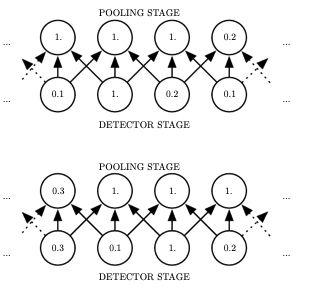
\includegraphics[width=0.5\linewidth]{Screen Shot 2021-01-18 at 11.33.20 AM.png}
        \caption{Every value in the bottom row has changed, but only half the values in the top row have changed. This details how pooling can be used to summarize the presence of something regardless of its location.}
        \label{fig:my_label}
    \end{figure}
    
    \item[$\bullet$] Can improve computation even more drastically be used fewer pooling units than detector units.
    
\end{description}

\end{document}

